\fontsize{13px}{13px}\selectfont\justifying

\chapter{TRIỂN KHAI VÀ ĐÁNH GIÁ}\label{section:dev}

\section{Triển khai}

\subsection{Cấu hình máy chủ}

\begin{itemize}
	\item \textbf{Máy chủ \gls{staging}} Virtual CPUs: 1. Memory (RAM): 2048 MB. Disk: 15 GB
	
	\item \textbf{Máy chủ \gls{production}}. Virtual CPUs: 1. Memory (RAM): 1536 MB. Disk: 15 GB
	
	\item \textbf{Máy chủ database}. Virtual CPUs: 1. Memory (RAM): 1536 MB. Disk: 15 GB
	
	\item \textbf{Máy chủ proxy}. Virtual CPUs: 1. Memory (RAM): 1536 MB. Disk: 15 GB
\end{itemize}
\subsection{Cài đặt tiến trình}


\subsubsection{Máy chủ \gls{staging}}
\begin{itemize}
	\item Tiến trình accounts chạy ở chế độ \gls{staging} kết nối với database test
	\item Tiến trình sellers chạy ở chế độ \gls{staging} kết nối với database test
	\item Tiến trình bloggers chạy ở chế độ \gls{staging} kết nối với database test
	\item Tiến trình gateway chạy ở chế độ \gls{staging} cung cấp giao diện quản lí mà sanbox để kiểm tra API.
\end{itemize}
\subsubsection{Máy chủ \gls{production}}
\begin{itemize}
	\item Tiến trình accounts chạy ở chế độ \emph{production} kết nối với database account
	\item Tiến trình  chạy ở chế độ \emph{production} kết nối với database seller
	\item Tiến trình bloggers chạy ở chế độ \emph{production} kết nối với database blogger
	\item Tiến trình gateway chạy ở chế độ \emph{production} cung cấp giao diện quản lí.
\end{itemize}

\subsubsection{Máy chủ database}
Cấu hình mongodb và cung cấp các database cho các môi trường phát hành.
\begin{itemize}
	\item account
	\item seller
	\item blogger
	\item test (cho môi trường \gls{staging})
\end{itemize}
\subsubsection{Máy chủ proxy}
Cấu hình liên kết tên miền với cổng tiến trình của các máy chủ trong hệ thống. Đăng ký chứng thực \acrshort{ssl}. Sử dụng các thuật toán cân bằng tải có sẵn để điều phối \gls{request}.

\subsection{Hình ảnh triển khai}
\FloatBarrier
\begin{figure}[!htbp]\fontsize{13px}{13px}\selectfont
\centering
		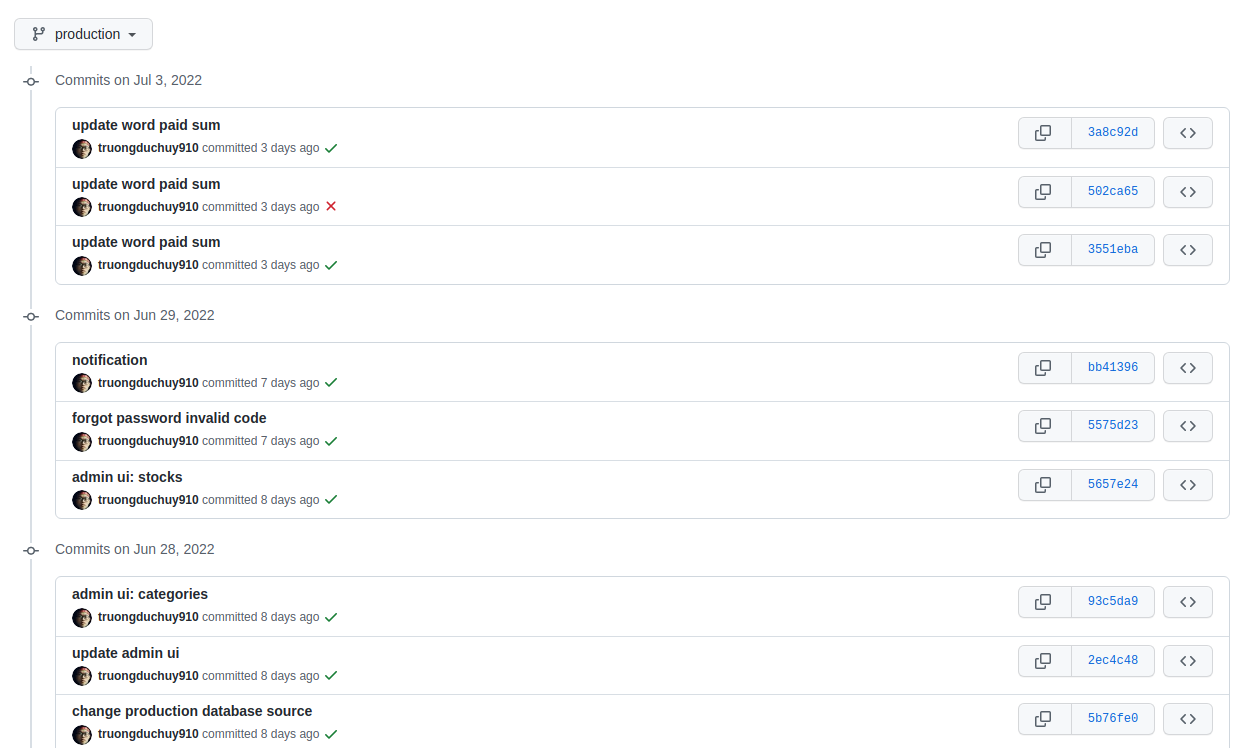
\includegraphics[width=\textwidth]{./results/commit}
		\caption{Lịch sử các phiên bản phát hành môi trường \gls{production}.}
\justifying
Các commit được triển khai thành công sẽ hiện dấu tích xanh. Khi có sự cố có thể quay về bản triển khai thành công trước đó. Là một phương án tốt khi có lỗ hổng trên môi trường \gls{production}.
	
\end{figure}
\clearpage
\FloatBarrier
\begin{figure}[!htbp]\fontsize{13px}{13px}\selectfont
\centering
		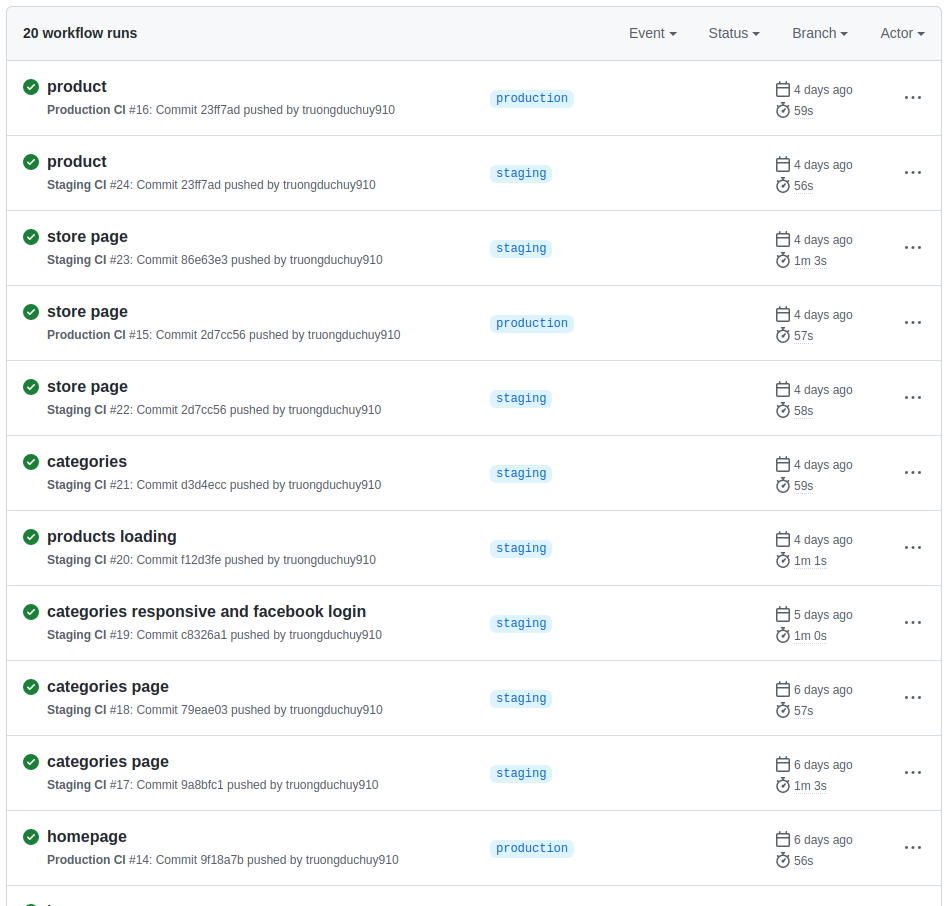
\includegraphics[width=\textwidth]{./results/deployments}
		\caption{Lịch sử cài đặt tiến trình ở các môi trường \gls{staging} và \gls{production} sử dụng CI/CD của github actions.}
\justifying
Lịch sử triển khai các commit trên các môi trường. Sau khi triển khai các tính năng trên môi trường \gls{staging} và trải qua công việc kiểm thử. Nếu không phát sinh vấn đề. Tất cả tính năng mới của \gls{staging} so với \gls{production} sẽ được triển khai bằng cách gộp mã nguồn của nhánh \gls{staging} vào nhánh \gls{production}.
	
\end{figure}
\clearpage
\begin{figure}[h!]\fontsize{13px}{13px}\selectfont
\centering
		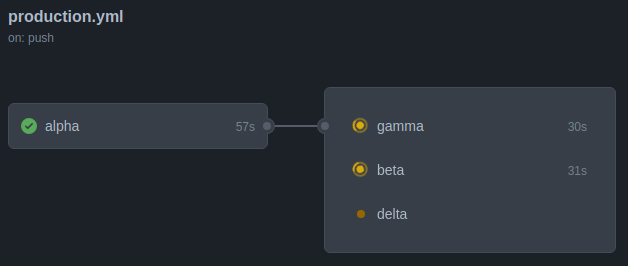
\includegraphics[width=\textwidth]{./results/jobs}
		\caption{Thông tin chi tiết khi sử dụng CI/CD chạy các bản sao của micro service trên nhiều máy chủ khác nhau}
\justifying
Hình trên mô tả máy chủ alpha là một máy chủ dự phòng của các máy chủ còn lại. Máy chủ alpha có khả năng dự phòng cho hầu hết các máy chủ dịch vụ khác. Nhưng ít khi được sử dụng. Khi việc triển diễn ra thành công trên máy chủ dự phòng, các máy chủ dịch vụ khác mới được triển khai để tránh trường hợp ảnh hưởng đến trải nghiệm phía người dùng.
\end{figure}


\begin{figure}[h!]\fontsize{13px}{13px}\selectfont
	\begin{center}	
		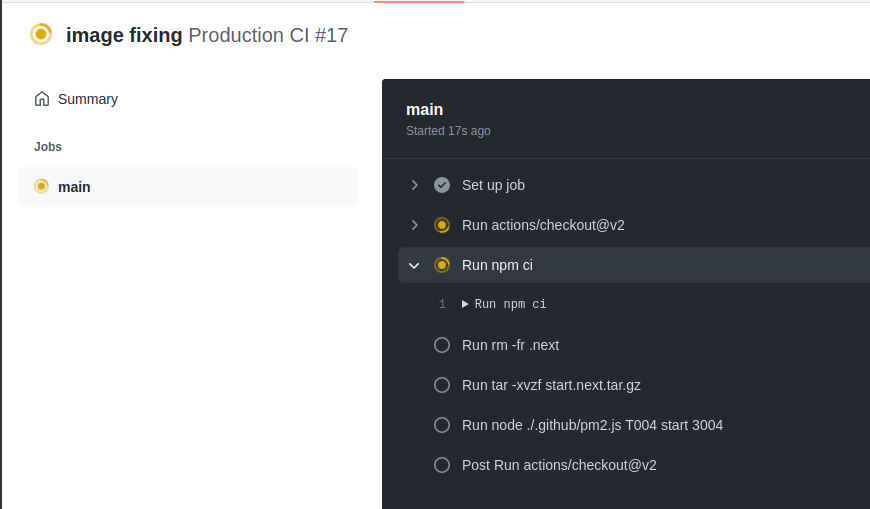
\includegraphics[width=\textwidth]{./results/production}
		\caption{Thông tin chi tiết các bước của một mirco-service sử dụng CI/CD}
	\end{center}
\end{figure}


